\chapter{Mensch-Roboter-Interaktion} %TODO

\section{Herausforderungen} %TODO
Was sind die Probleme, die mit der Anwendung gelöst werden sollen? Was waren die Hindernisse, die sich für diese Arbeit gestellt haben? 

\section{Stand der Technik} %TODO
Werden ähnliche Tools bereits eingesetzt, wenn ja mit welchem Erfolg? Was war der bisherige Ansatz in dieser Domäne (Pepper-Programmierung)?

\section{Kollaborations-Schnittstelle} %TODO
Was ergibt sich aus 2.1 und 2.2 für die Arbeit? Welche grobe Zielsetzung wurde festgelegt?





\begin{figure} %TODO Löschen, wenn erstes Bild eingefügt
	\centering
	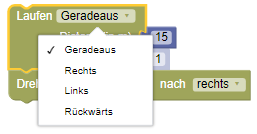
\includegraphics[width=5cm]{Plots/zz-placeholder.png}
	\caption{Platzhalter für Abbildungsverzeichnis.}
	\label{fig:placeholder}
\end{figure}